\documentclass{beamer}

\usepackage{Haust2016glærur}

\title{Tölvunarfræði 1a}
\subtitle{Vika 7, fyrri fyrirlestur}

\begin{document}

\begin{frame}
\titlepage
\end{frame}

\section{Inngangur}

\begin{frame}{Í síðasta þætti\ldots}
\begin{itemize}
 \item Aflúsun
 \item Fleytitölur
\end{itemize}
Kafli: 6.5
\end{frame}

\section{Strengir}

\begin{frame}{Strengir}
\begin{itemize}
 \item Mörg forritunarmál hafa sérstak tag fyrir strengi
 \begin{itemize}
  \item Matlab hefur það ekki
 \end{itemize}
 \item Í Matlab eru strengir línuvigrar með stökum af taginu \texttt{char}
 \begin{itemize}
  \item Það eru sérstök föll í Matlab sem vinna með strengi
  \item En þar sem strengir eru vigrar þá er líka hægt að nota flest vigurföllin
 \end{itemize}
\end{itemize}
\end{frame}

\begin{frame}[fragile]{Strengjafastar}
\begin{itemize}
 \item Þó að strengir séu vigrar þá líta strengjafastar ekki neitt sérstaklega mikið út eins og vigrar
 \begin{itemize}
  \item Byrja og enda á einfaldri gæsalöpp
 \end{itemize}
\begin{minted}[frame=lines]{matlab}
>> 'Halló';
>> 'a';
>> '123'; % Strengur inniheldur tölu
>> ''; % Tómi strengurinn
>> 'strengur með eyðum';
\end{minted}
\end{itemize}
\end{frame}

\begin{frame}{Strengir innihalda stafi}
\begin{itemize}
 \item Stafir geta verið af ýmsum gerðum:
 \begin{itemize}
  \item Bókstafir \texttt{'a', 'B', 'ó', 'Þ'}, \ldots
  \item Tölustafir \texttt{'0', '1', '2',} \ldots
  \item Greinarmerki \texttt{'.', ':', ';', '?'}, \ldots
  \item Biltákn (e. \emph{whitespace})	eyða, tab, ný-lína, \ldots
  \item Stýritákn (e \emph{control characters})	óprentanleg tákn 
 \end{itemize}
\end{itemize}
\end{frame}

\begin{frame}{ASCII}
\begin{center}
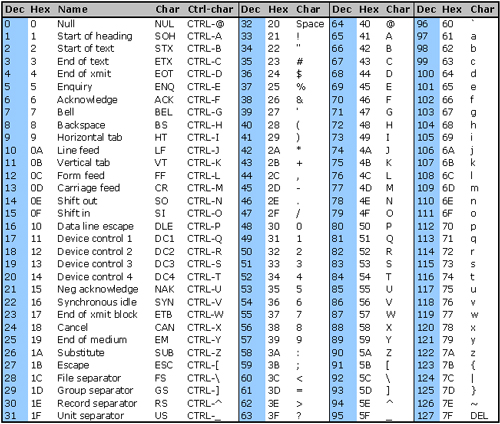
\includegraphics[width=0.8\textwidth]{Pics/ascii-full}
\end{center}
\end{frame}

\begin{frame}[fragile]{Að breyta á milli stafa og talna}
\begin{minted}[frame=lines]{matlab}
>> double('a') % líka hægt að nota int32 o.fl.
ans =  97
>> char(97) % Breytir ASCII talnakóða í táknið
ans = a
>> num2str(2) % Breytir tölu í tilsvarandi char
ans = 2
>> str2num('2') % Breytir streng í double
ans =  2
\end{minted}
\end{frame}

\begin{frame}[fragile]{Að búa til strengjabreytur}
\begin{columns}
\column{0.3\textwidth}
\begin{itemize}
 \item Að nota gildisveitingu
 \item Lesa inn í breytu með \texttt{input}-falli
\end{itemize}\pause
\column{0.7\textwidth}
\begin{minted}[frame=lines]{matlab}
>> text = 'Yes, this is dog';
>> name = input('Sláið inn nafn: ', 's')
Sláið inn nafn: DOG
name = DOG
>> name2 = input('Sláið inn nafn: ', 's')
Sláið inn nafn:      DOG
name2 =      DOG
\end{minted}
\end{columns}
\end{frame}

\begin{frame}[fragile]{Strengir eru vigrar}
\begin{columns}
\column{0.5\textwidth}
\begin{itemize}
 \item Í Matlab eru strengir vigrar af bókstöfum
 \item Við getum unnið með strengi eins og vigra
 \begin{itemize}
  \item Náð í einstaka stafi
  \item Beitt vigurföllum
  \item Unnið með hlutstrengi
 \end{itemize}

\end{itemize}
\pause
\column{0.5\textwidth}
\begin{minted}[frame=lines]{matlab}
>> s = ['a', 'b', 'c'];
>> s(2)
ans = b
>> length(s)
ans =  3
>> t = 'Annar strengur';
>> t(3:5)
ans = nar
\end{minted}
\end{columns}
\end{frame}

\begin{frame}[fragile]{Strengir eru vigrar}
\begin{columns}
\column{0.5\textwidth}
\begin{itemize}
 \item Getum búið til stafafylki
 \begin{itemize}
  \item Þá er einn strengur í hverri línu fylkisins
  \item Til hægri: $2 \times 5$ fylki af stöfum
 \end{itemize}
\end{itemize}

\column{0.5\textwidth}
\begin{minted}[frame=lines]{matlab}
>> names = ['Nonni';'Jonni']
names =
Nonni
Jonni
\end{minted}
\pause
Galli: Allar línur í stafafylki þurfa að vera jafn langar!
\end{columns}
\end{frame}

\begin{frame}{Samskeyting strengja}
\begin{itemize}
 \item Tvær leiðir færar til að skeyta saman strengjum
 \begin{enumerate}
  \item Skeyta saman eins og (öðrum) vigrum
  \item Nota samskeytingarfallið \texttt{strcat}
  \begin{itemize}
   \item \texttt{strcat} = \textbf{str}ing con\textbf{cat}enation
  \end{itemize}  
 \end{enumerate}
 \item Biltákn eru meðhöndluð á mismunandi hátt í lok strengja
 \begin{itemize}
  \item Vigursamskeytingin varðveitir allar eyður í samskeytingunni
  \item Fallið \texttt{strcat} hendir út eyðum aftast í báðum strengjunum
 \end{itemize}
\end{itemize}
\end{frame}

\begin{frame}{Fyrirlestraræfing}
Skráið ykkur inn á \url{http://socrative.com/} og gerið fyrstu tvær spurningarnar.

Herbergisnúmer = \texttt{TOL105G2016}

Notendanafn = HÍ-tölvupóstfang
\end{frame}

\subsection{Strengjaföll og sérsmíðun}

\begin{frame}{Að sérsmíða strengi}
\vspace{\baselineskip}
Stundum þurfum við strengi með mjög ákveðna uppbyggingu. Gagnleg föll:
\begin{center}
\begin{tabular}{lp{7cm}}
\toprule
Fall&Merking\\
\midrule
\texttt{blanks}&Býr til streng með tiltekinn fjölda eyða\\
\texttt{sprintf}&Virkar alveg eins og \texttt{fprintf}, nema það býr til streng í stað þess að prenta\\
\texttt{deblank}&Hendir eyðum aftast í strengjum\\
\texttt{strtrim}&Hendir eyðum framan og aftan af streng (ekki inni í honum)\\
\bottomrule
\end{tabular}
\end{center}
\end{frame}

\begin{frame}[fragile]{Önnur strengjaföll}
\begin{center}
\begin{tabular}{ll}
\toprule
Fall&Merking\\
\midrule
\texttt{upper}&Býr til streng með eingöngu hástöfum\\
\texttt{lower}&Býr til streng með eingöngu lágstöfum\\
\texttt{strcat}&``Lárétt'' strengjasamskeyting\\
\texttt{strvcat}&``Lóðrétt'' strengjasamskeyting\\
\bottomrule
\end{tabular}
\end{center}
\end{frame}

\begin{frame}[fragile]{Is-föll fyrir strengi}
\begin{center}
\begin{tabular}{ll}
\toprule
Fall&Merking\\
\midrule
\texttt{isletter}&Satt ef stafur (char) er bókstafur\\
\texttt{isspace}&Satt ef stafur er biltákn\\
\texttt{ispunct}&Satt ef stafur er greinarmerki\\
\texttt{ischar}&Satt ef gefin breyta er af taginu \texttt{char}\\
\bottomrule
\end{tabular}
\end{center}

\end{frame}


\subsection{Samanburður strengja}

\begin{frame}[fragile]{Samanburður strengja}
Vegna þess að strengir eru vigrar er venjulegur samanburður framkvæmdur ``stak fyrir stak'':
\begin{minted}[frame=lines]{matlab}
>> s1 = 'Nonni'; s2 = 'nonni';
>> s1 == s2
ans =
   0   1   1   1   1
\end{minted}
Hægt er að nota \texttt{all(s1==s2)}, en þá þurfa strengirnir að vera jafn langir.
\end{frame}

\begin{frame}[fragile]{Fall til strengjasamanburðar}
\begin{itemize}
 \item Fallið \texttt{strcmp} ber saman strengi
 \begin{itemize}
  \item Skilar ``satt'' ef þeir eru alveg eins
  \item Skilar ``ósatt'' ef þeir eru mislangir eða ekki eins
 \end{itemize}
\end{itemize}
\begin{minted}[frame=lines]{matlab}
>> s1 = 'Nonni'; s2 = 'nonni';
>> strcmp(s1, s2)
ans = 0
\end{minted}
\end{frame}

\begin{frame}{Föll til strengjasamanburðar}
\vspace{\baselineskip}
\begin{center}
\begin{tabular}{lp{8cm}}
\toprule
Fall&Merking\\
\midrule
\texttt{strcmp}&Athugar hvort tveir strengir séu eins, hástafir og lágstafir aðskildir\\
\texttt{strcmpi}&Athugar hvort tveir strengir séu eins, hástafir og lágstafir álitnir eins\\
\texttt{strncmp}&Athugar hvort fyrstu n stafirnir í strengjum séu eins, hástafir og lágstafir aðskildir\\
\texttt{strncmpi}&Athugar hvort fyrstu n stafirnir í strengjum séu eins, hástafir og lágstafir álitnir eins\\
\bottomrule
\end{tabular}
\end{center}
\end{frame}

\subsection{Leit og útskipting}

\begin{frame}[fragile]{Leit í strengjum}
\begin{itemize}
 \item Fallið strfind tekur tvo strengi og leitar að seinni strengnum í þeim fyrri og skilar staðsetningu hans
 \begin{itemize}
  \item Ef seinni strengurinn kemur oft fyrir þá er úttakið vigur
 \end{itemize}
\end{itemize}
\begin{minted}[frame=lines]{matlab}
>> strfind('abracadabra','bra')
ans =
     2    9
\end{minted}
\end{frame}

\begin{frame}[fragile]{Að skipta út strengjum}
Fallið \texttt{strrep(str,h1,h2)} finnur öll tilvik af \texttt{h1} í \texttt{str} og skiptir þeim út fyrir \texttt{h2}.
\begin{minted}[frame=lines]{matlab}
>> strrep('abcdeabcde','e','x')
ans = abcdxabcdx
\end{minted}
\end{frame}

\begin{frame}{Fyrirlestraræfing}
Skráið ykkur inn á \url{http://socrative.com/} og klárið spurningarnar.

Herbergisnúmer = \texttt{TOL105G2016}

Notendanafn = HÍ-tölvupóstfang
\end{frame}



\end{document}
